\section{Arrays of $10^4$ to $10^6$ sites}\label{sec:megascale}

We ask what limits an array of $10^4$, $10^5$ or $10^6$ sites at 3 to 4~\textmu m pitch, in the order in which the limits appear, and what the transport hardware of the previous chapters must look like to assemble such an array and keep it filled. The record is \texttt{docs/\allowbreak megascale.md} (Secs.~1 to 10); the code is \texttt{scripts/m22\_megascale.py} (budget, tiling), \texttt{picsim/megasort.py} with \texttt{scripts/m23\_steady.py} (assembly and steady state), \texttt{scripts/m24\_tiling\_wave.py} and \texttt{scripts/m25\_imaging.py}.

The short answer is as follows. At 4~\textmu m pitch the transport side scales to $10^6$ sites. An engine block of 32 rows $\times$ 4 engines (128 engines) assembles $10^6$ sites from 85\% loading to $10^{-3}$ defects in 1.0 to 1.1~s with fast handoff steps, and then holds the array at a time-averaged defect fraction of $1.8\times10^{-4}$ ($2.4\times10^{-4}$ sampled at the image). Three walls come first: (i) the corrected field of the objective, (ii) the static trapping power, which is the first wall at $10^6$ sites, and (iii) the loss rates (vacuum lifetime and loss per image), which set the steady-state floor at every array size. At $10^6$ sites the transport adds a fourth constraint, the latency of a block that must sweep 252 positions to reach a hole; it is removed by fast steps, a larger block, or a slower imaging cadence. Table~\ref{tab:mega-overview} collects the scale-dependent numbers.

\begin{table}[htbp]\centering\small
\caption{Scale of the problem (derived, \texttt{results/\allowbreak m22\_budget.json}). Field radius $L/\sqrt{2}$ for a square of side $L$; resolution cell 1.06~\textmu m at NA 0.5; static power at 4.5~mW per site per mK, 85\% loading including the reservoir; block positions for the 32~$\times$~4 block at 4~\textmu m pitch; refills for $\tau=3000$~s and $\epsilon_\mathrm{img}=10^{-4}$ at 10~Hz imaging.}
\label{tab:mega-overview}
\begin{tabular}{lccc}
\toprule
 & $10^4$ sites & $10^5$ sites & $10^6$ sites \\
\midrule
side at 4 / 3~\textmu m pitch & 0.40 / 0.30~mm & 1.26 / 0.95~mm & 4.0 / 3.0~mm \\
single objective: field radius (4~\textmu m) & 0.28~mm & 0.89~mm & 2.8~mm \\
resolution cells per side (4~\textmu m) & 372 & 1,187 & 3,754 \\
zones of $\pm250$~\textmu m (objectives) & 2 & 13 & 127 \\
static power at the atoms, 0.1 / 1~mK & 5.3 / 53~W & 53 / 530~W & 0.53 / 5.3~kW \\
32~$\times$~4 block: positions & 10 & 28 & 252 \\
refills needed per second & 13 & 134 & 1,335 \\
\bottomrule
\end{tabular}
\end{table}

\subsection{The walls in order}\label{sec:megascale-walls}

\paragraph{Field and space-bandwidth.} A square array of side $L$ needs a corrected field of radius $L/\sqrt{2}$. At 4~\textmu m pitch that is 372, 1,187 and 3,754 resolution cells per side for $10^4$, $10^5$ and $10^6$ sites; the last corresponds to a space-bandwidth product of about $1.4\times10^7$. The $\pm100$~\textmu m field of the proposal~\cite{proposal} covers none of these. $10^4$ sites need $\pm0.28$~mm. $10^5$ sites need $\pm0.9$~mm, which is within the range of refractive NA 0.5 objectives (recalled, to be verified). $10^6$ sites need a lithography-class field of $\pm2.8$~mm at NA 0.5. Zones, i.e.\ independent arrays each with its own objective, static array and engine block, avoid the large field. A $\pm250$~\textmu m zone holds 7,700 sites at 4~\textmu m and assembles like the $10^4$ case. However, each zone needs its own objective, about 25 to 30~mm across at a 15~mm working distance, so the 127 zones needed for $10^6$ sites are impractical. Zones therefore suit $10^4$ (2 zones) to $10^5$ sites (13 zones); at $10^6$ a single large-field objective, or a few large zones, cannot be avoided.

\paragraph{Static trapping power.} From the trap depth with $\alpha(1075~\mathrm{nm})=1120$~au and a 0.85~\textmu m waist, a tweezer needs 4.5~mW per site per mK at the atoms. The reservoir sites count as well. The budget of Table~\ref{tab:mega-overview} uses the minimum reservoir fraction $1-f$, i.e.\ 50\% of all sites at 50\% loading and 15\% at 85\%; the simulated 3:1 layout at 85\% uses 25\%, which adds 13\% to these powers. At the 0.1~mK hold of the transport model (Sec.~\ref{sec:transport}), $10^6$ sites take 0.5 to 0.9~kW at the atoms (85\% to 50\% loading), and 5 to 9~kW at a 1~mK loading or imaging depth. With an assumed delivery efficiency of 30\%, the laser must supply 1.8 to 3~kW at the hold and 18 to 30~kW at 1~mK. This is the first wall at $10^6$ sites.

An optical lattice is the obvious alternative for the static potential, as in the continuously operated lattice array of Gyger et al.~\cite{gyger2024} (known to us from a search summary only). Table~\ref{tab:mega-static} compares the two (derived, \texttt{results/\allowbreak m22\_lattice.json}). The lattice uses two orthogonal retro-reflected beams (incoherent sum, peak $8I$ per beam; coherent four-beam sum, $16I$), held within $-20\%$ of the peak over the array. A tweezer puts its power into about $\pi w_0^2/2=1.1$~\textmu m$^2$ per site. A Gaussian lattice beam that keeps the corners within 20\% spreads it over about $15a^2/G=31$~\textmu m$^2$. Hence a free-space lattice loses to tweezers by about 25 with Gaussian beams and by 2 to 4 with flat-top beams. Only an enhancement cavity with a buildup near 100 wins, by a factor of about 4, and that cavity would need a waist near 10~mm for $10^6$ sites. Two levers do more than the choice of potential: the depth (a factor of 10 between 1 and 0.1~mK), and the delivery efficiency, which for the simpler lattice optics could gain up to about 2.7 (0.8 instead of 0.3). For $10^6$ sites the static potential thus needs about 2~kW of laser power at the hold depth with tweezers, or about 0.5~kW with a buildup-100 cavity lattice, and loading and imaging must happen at a lower depth or in a smaller zone.

\begin{table}[htbp]\centering\small
\caption{Laser power for the static potential at 30\% delivery (assumed), for $N$ sites plus a 25\% reservoir at 4~$\times$~4~\textmu m, at depths of 0.1 / 1~mK (derived, \texttt{results/\allowbreak m22\_lattice.json}). Lattices: two orthogonal retro-reflected beams held within $-20\%$ of the peak; cavity buildup is a choice.}
\label{tab:mega-static}
\begin{tabular}{lccc}
\toprule
static potential & $10^4$ sites & $10^5$ sites & $10^6$ sites \\
\midrule
tweezer array ($w_0=0.85$~\textmu m) & 20 / 200~W & 0.2 / 2.0~kW & 2.0 / 20~kW \\
free-space lattice, Gaussian beams & 0.5 / 5.0~kW & 5 / 50~kW & 50 / 500~kW \\
free-space lattice, flat-top, incoherent & 85~W / 0.85~kW & 0.85 / 8.5~kW & 8.5 / 85~kW \\
free-space lattice, flat-top, coherent & 42~W / 0.42~kW & 0.42 / 4.2~kW & 4.2 / 42~kW \\
cavity lattice, Gaussian, buildup 10 & 50~W / 0.5~kW & 0.5 / 5~kW & 5 / 50~kW \\
cavity lattice, Gaussian, buildup 100 & 5 / 50~W & 0.05 / 0.5~kW & 0.5 / 5~kW \\
\bottomrule
\end{tabular}
\end{table}

\paragraph{Engines, blocks and tiling along $x$.} One engine (192 ports, 383 fast actuators, Sec.~\ref{sec:engine}) serves a 180~\textmu m row segment, i.e.\ 45 to 46 sites at 4~\textmu m and 60 to 61 at 3~\textmu m. Engines can be tiled in two directions. Along $y$, chips are stacked, one chip per row with its own collimator (Sec.~\ref{sec:rows}). Along $x$, several engines share one chip edge: each gets its own $x$ lenslet, and a common Fourier lens overlaps all of them in the pupil and maps their offsets to adjacent atom segments. The ABCD check (\texttt{m22\_tiling}) gives a magnification of $-60.1$ for every engine and all chief rays at the pupil centre. The question is how close the engines can sit. A first-order argument gave a pessimistic answer: with 1.5~\textmu m emitter pitch, each engine's first grating lobe lands 204~\textmu m from its spot at the atoms, inside the neighbouring segment, so a shared slit plane would need opaque gaps as wide as the slit zones, and hence an engine pitch $P_e\geq4.4$~mm (four engines per 18~mm edge).

The wave-optics check (\texttt{results/\allowbreak m24\_tiling\_wave.json}) supersedes this. We propagate the emitter near field of one D1 engine, forming a tweezer at $x_a=0$, 60 and 90~\textmu m (up to the segment edge), over $f_1=3.12$~mm to its lenslet (clear aperture equal to fill $\times P_e$), apply an ideal lens phase, propagate over $f_1$ to the shared slit plane $\Sigma$, and measure the intensity in the neighbouring engine's slit zone. Here, $\Sigma$ is conjugate to the atoms, so this intensity is the ghost that a neighbouring segment sees. We keep only directions inside the pupil acceptance $A/(2f_1)$, because steeper light misses the objective, and an exact ray trace through the neighbouring lenslets checks the same question geometrically. Table~\ref{tab:mega-tiling} and Fig.~\ref{fig:mega-tiling} give the result. The first-order lobes are not the limit: the lenslet aperture and the pupil acceptance remove them, and no accepted ray reaches another slit zone at any pitch scanned. What sets the pitch is the lenslet aperture needed to pass the engine's own slit zone, $2f_1\tan(\arcsin s_\mathrm{cut})=2.37$~mm. Below 2.6~mm the lenslet clips the engine's own beam and its diffraction tail enters the neighbouring zone. At $P_e=3.0$~mm the accepted ghost is below $2\times10^{-7}$ of a tweezer peak, under the coherent criterion of $10^{-6}$ (\texttt{docs/\allowbreak row\_coherence.md}). Hence six engines fit on an 18~mm chip edge instead of four. Two scanner positions per row are still needed: the segment pitch at the atoms, $P_e f_\mathrm{obj}/f_c=0.092\,P_e=277$~\textmu m at $P_e=3.0$~mm ($f_c=188$~mm, $f_\mathrm{obj}=17.3$~mm), exceeds the 180~\textmu m segment, so one block position addresses every other segment. The model is 1D ($x$ only) with an ideal thin lens and no surface scatter; baffles between the lenslet channels remain the defence against scattered light, which it does not include.

\begin{table}[htbp]\centering\small
\caption{Ghost of one engine in its neighbour's slit zone versus engine pitch $P_e$ (simulated, 1D, \texttt{results/\allowbreak m24\_tiling\_wave.json}). Worst case over $x_a=0$, 60, 90~\textmu m at lenslet fill 1 (the segment-edge tweezer, except at 3.5~mm where $x_a=60$~\textmu m is marginally worse). ``Accepted'' keeps only directions inside the pupil acceptance. A fill of 0.8 at 4.43~mm raises the accepted ghost to $2\times10^{-9}$. No accepted ray through a neighbouring lenslet reaches another slit zone at any pitch.}
\label{tab:mega-tiling}
\begin{tabular}{lccc}
\toprule
 & \multicolumn{2}{c}{ghost peak / tweezer peak} & ghost power / \\
$P_e$ & accepted & raw & own slit power \\
\midrule
8.0~mm & $4.5\times10^{-13}$ & $1.7\times10^{-9}$ & $2.6\times10^{-13}$ \\
4.43~mm & $3.6\times10^{-10}$ & $2.5\times10^{-7}$ & $1.4\times10^{-10}$ \\
3.5~mm & $1.7\times10^{-8}$ & $3.1\times10^{-6}$ & $1.0\times10^{-8}$ \\
3.0~mm & $1.7\times10^{-7}$ & $7.7\times10^{-6}$ & $6.3\times10^{-8}$ \\
2.6~mm & $1.6\times10^{-6}$ & $1.3\times10^{-5}$ & $7.5\times10^{-7}$ \\
2.4~mm & $6.7\times10^{-5}$ & $5.6\times10^{-5}$ & $7.2\times10^{-5}$ \\
\bottomrule
\end{tabular}
\end{table}

\begin{figure}[htbp]\centering
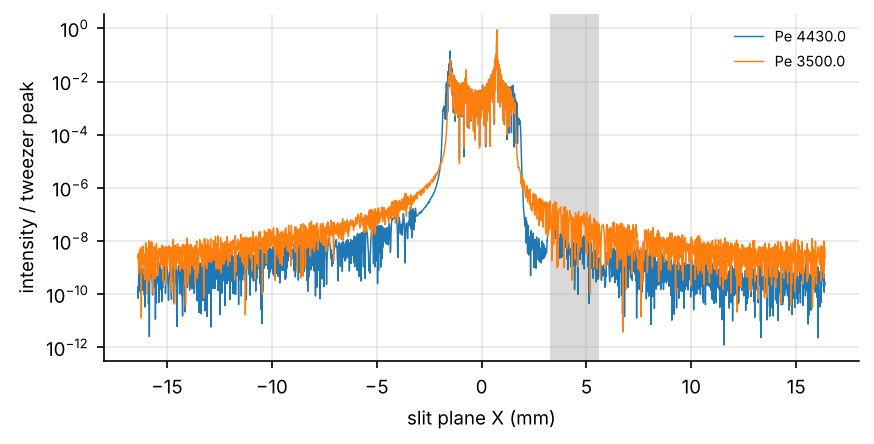
\includegraphics[width=0.8\linewidth]{m24_tiling_wave.png}
\caption{Intensity at the shared slit plane $\Sigma$, relative to the tweezer peak, for one D1 engine forming a tweezer at the segment edge ($x_a=90$~\textmu m), lenslet fill 1, engine pitch 4.43~mm (blue) and 3.5~mm (orange). 1D angular-spectrum propagation of the emitter near field over $f_1=3.12$~mm, ideal lens phase on the lenslet aperture, and propagation over $f_1$ (0.25~\textmu m grid). The grey band is the neighbouring engine's slit zone at 4.43~mm pitch, $|X-P_e|<f_1 s_\mathrm{cut}$. The curves show the raw intensity, before the pupil-acceptance filter applied in Table~\ref{tab:mega-tiling}.}
\label{fig:mega-tiling}
\end{figure}

A block of 32 rows (two 16-chip stacks, combined by polarisation or by the comb of Sec.~\ref{sec:combine}) $\times$ 4 engines per row has 128 engines and 49,024 fast actuators. It holds 5,888 simultaneous tweezers, which need 85~W at 0.3~mK if all are lit; that happens at most during assembly, since in steady state only the few refilling tweezers are lit. A single 16-chip stack (a 16~$\times$~1 block) is too small for $10^6$ sites: it never finishes assembling.

\paragraph{Pitch.} At 3~\textmu m pitch in both directions the transport lane passes 1.5~\textmu m from waiting atoms, and the moving tweezer pulls most of them out, so such a lattice would need empty corridor rows. The anisotropic lattice avoids this (Sec.~\ref{sec:transport}): with 3~\textmu m along the rows and rows 4~\textmu m apart, the lane stays 2~\textmu m from the rows and the lattice transports as cleanly as 4~$\times$~4~\textmu m. It has 33\% more sites per area (0.063 against 0.047 computation sites per \textmu m$^2$ with a 3:1 reservoir layout). Below, ``3~\textmu m'' means this 3~$\times$~4~\textmu m lattice.

\subsection{Assembly and steady-state refilling}\label{sec:megascale-steady}

The simulation (\texttt{picsim/megasort.py}) represents the array as computation rows interleaved with reservoir rows (1:2 at 50\% loading, 3:1 at 85\%). The array is imaged every $T_\mathrm{img}=0.1$~s for $t_\mathrm{img}=10$~ms, with a loss $\epsilon_\mathrm{img}=10^{-4}$ per image and $10^{-4}$ per move; the reservoir is refreshed every 1~s from an external supply. The engine block visits, round-robin, the tiles with known holes, and each visit runs up to four repair passes (a common row shift, an order-preserving $x$ pass, and one move per refill). Two step timings come from the rearrangement chapter (Sec.~\ref{sec:rearrange}): slow (200~\textmu s ramps, 400~\textmu s lane steps, 0.2 to 0.3~\textmu K per move) and fast (50~\textmu s ramps, 100~\textmu s lane steps, 200~\textmu s per 40~\textmu m, about 1 to 10~\textmu K per move). Table~\ref{tab:mega-assembly} and Fig.~\ref{fig:mega-steady} summarise the runs at 4~\textmu m pitch. Their steady-state values are sampled just after an image; Sec.~\ref{sec:megascale-defects} explains why the time average is lower.

\begin{table}[htbp]\centering\small
\caption{Assembly and steady state at 4~\textmu m pitch (simulated, \texttt{results/\allowbreak m23\_steady.json}). Time from a random loading to $10^{-2}$ and $10^{-3}$ defects (n.r.: not reached in 20~s), and the steady-state defect fraction sampled just after each image, in units of $10^{-4}$, for $\tau=3000$ / 300~s. Slow and fast step timings as in the text. At $10^6$ sites with $\tau=300$~s, slow steps do not reach $10^{-3}$.}
\label{tab:mega-assembly}
\begin{tabular}{llllccc}
\toprule
sites & loading & block & timing & to $10^{-2}$ & to $10^{-3}$ & steady state, $\tau$ 3000 / 300~s \\
\midrule
$10^4$ & 50\% & 16$\times$1 & slow & 0.34~s & 0.34~s & 2.7 / 5.6 \\
$10^4$ & 50\% & 32$\times$4 & slow & 0.12~s & 0.12~s & 2.6 / 5.6 \\
$10^4$ & 85\% & 32$\times$4 & slow & 0.12~s & 0.12~s & 1.8 / 5.7 \\
$10^5$ & 50\% & 16$\times$1 & slow & 1.8~s & 1.8--2.8~s & 2.3 / 6.0 \\
$10^5$ & 50\% & 32$\times$4 & slow & 0.46~s & 0.46~s & 2.5 / 6.1 \\
$10^5$ & 85\% & 32$\times$4 & slow & 0.24~s & 0.24~s & 2.5 / 5.8 \\
$10^5$ & 85\% & 32$\times$4 & fast & 0.12~s & 0.12~s & 2.5 ($\tau$ 3000~s) \\
$10^6$ & 50\% & 32$\times$4 & slow & 2.2~s & 2.8~s ($\tau$ 3000~s) & 8.6 / 32 \\
$10^6$ & 85\% & 32$\times$4 & slow & 1.9~s & 3.1~s ($\tau$ 3000~s) & 9.3 / 38 \\
$10^6$ & 85\% & 32$\times$4 & fast & 0.79~s & 1.1~s & 2.4 ($\tau$ 3000~s) \\
$10^6$ & 50\% / 85\% & 16$\times$1 & slow & 14~s ($\tau$ 3000~s) & n.r. & 70 to 290 \\
\bottomrule
\end{tabular}
\end{table}

\begin{figure}[htbp]\centering
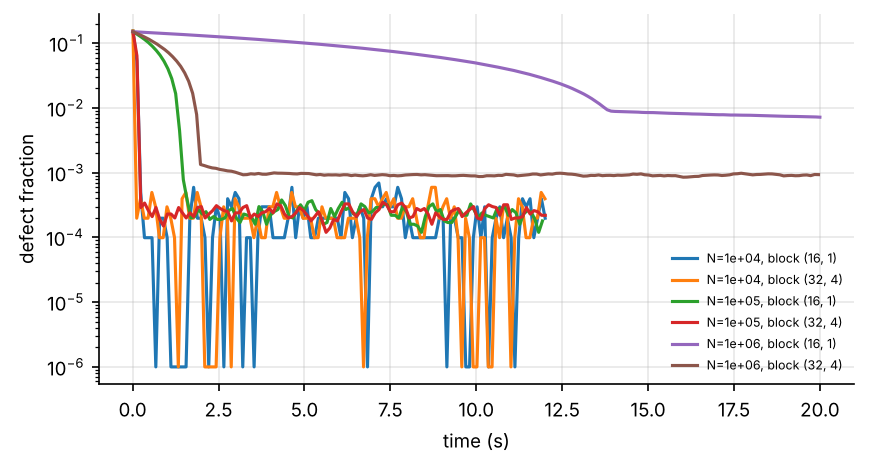
\includegraphics[width=0.8\linewidth]{m23_steady.png}
\caption{Defect fraction sampled just after each image versus time, from a random 85\% loading (3:1 computation to reservoir rows) at 4~\textmu m pitch, slow steps, $\tau=3000$~s, $\epsilon_\mathrm{img}=10^{-4}$ per image and per move, imaging every 0.1~s, for blocks of 16~$\times$~1 and 32~$\times$~4 engines and $10^4$ to $10^6$ sites (\texttt{scripts/m23\_steady.py}). Values of zero are drawn at $10^{-6}$. With slow steps, $10^6$ sites with the 32~$\times$~4 block settle at the latency-limited $9\times10^{-4}$, and the 16~$\times$~1 block does not reach $10^{-3}$. Fast steps (not shown) restore the loss-limited floor.}
\label{fig:mega-steady}
\end{figure}

Three findings follow. (i) Up to $10^5$ sites the floor is set by the losses, and it is nearly the same for every block and timing (1.7 to $2.7\times10^{-4}$ at image for $\tau=3000$~s, the spread being run-to-run noise). (ii) At $10^6$ sites latency matters: with slow steps a sweep of 252 block positions takes longer than the imaging period, new holes wait several sweeps, and the floor rises about four-fold. Fast steps restore the loss-limited floor. (iii) Each refill is a single move from a nearby reservoir row into the hole, so heating does not accumulate on any atom. In steady state at $10^6$ sites the reservoir is consumed at about 1,300 atoms per second ($\tau=3000$~s). Chiu et al.~\cite{chiu2025} (abstract read) report 30,000 initialized qubits per second from lattice conveyor belts, maintaining more than 3,000 atoms for over 2 hours; that rate would cover our demand with a margin of 20. For comparison with our loss parameters, Manetsch et al.~\cite{manetsch2024} (abstract read) report a 23~min lifetime in a room-temperature apparatus and 99.98952\% imaging survival ($\epsilon_\mathrm{img}=1.05\times10^{-4}$) for a 6,100-atom Cs tweezer array, i.e.\ close to our nominal $\epsilon_\mathrm{img}$ and a lifetime between our 300~s and 3000~s cases.

\subsection{Three defect fractions}\label{sec:megascale-defects}

The values of Table~\ref{tab:mega-assembly} are sampled just after each image. That value counts imaging losses twice. An image removes a fraction $\epsilon_\mathrm{img}$ of the atoms after detecting them, so these holes stay unseen for a full period, and at the next image they are still present when the new losses are added. The simulator therefore also records the value just before each image and the time average. The time average is a trapezoid sum over visit, image and idle intervals; it is exact in expectation for the vacuum losses, which are uniform in time, while each visit's fills are booked at its start, which biases the average low by at most one visit time (1 to 2~ms against $T_\mathrm{img}=100$~ms). The time average is what a computation started at a random moment sees. With fast steps at $10^6$ sites the three values are $2.4\times10^{-4}$ (at image), $1.4\times10^{-4}$ (before image) and $1.8\times10^{-4}$ (time average). The at-image value is close to $2\epsilon_\mathrm{img}+(T_\mathrm{img}+t_\mathrm{img})/\tau=2.4\times10^{-4}$, and the time average is close to $\epsilon_\mathrm{img}+(T_\mathrm{img}+t_\mathrm{img})/(2\tau)=1.2\times10^{-4}$ plus the repair latency. Thus the time average is about 25\% below the at-image figures quoted in Table~\ref{tab:mega-assembly}, and an earlier rule $\rho\approx(1.5\text{ to }1.8)(\epsilon_\mathrm{img}+T_\mathrm{img}/\tau)$, fitted to at-image values over a narrower range, is replaced by the fits of Sec.~\ref{sec:megascale-imaging}.

\subsection{Remedies at \texorpdfstring{$10^6$}{10\textasciicircum 6} sites}\label{sec:megascale-remedies}

At $10^6$ sites the choice is between a larger block and faster, hotter steps. We scanned blocks of 128 to 256 engines and three step timings with heating per move of 10~\textmu K (fast), 2~\textmu K (intermediate) and 0.3~\textmu K (slow), at 85\% loading, $\tau=3000$~s, $\epsilon_\mathrm{img}=10^{-4}$, $T_\mathrm{img}=100$~ms and rows 4~\textmu m apart (\texttt{results/\allowbreak m23\_remedy.json}, one seed per case). The intermediate timing (100~\textmu s ramps, 200~\textmu s lane steps) transports cleanly on the 3~$\times$~4~\textmu m lattice at 1 to 3~\textmu K per move with no bystander lost or displaced (\texttt{results/\allowbreak m18\_midlane.json}, 3,000 atoms per case; Sec.~\ref{sec:transport}); we use 2~\textmu K per move. Table~\ref{tab:mega-remedy} gives the results.

\begin{table}[htbp]\centering\small
\caption{Remedies at $10^6$ sites (simulated, \texttt{results/\allowbreak m23\_remedy.json}; 85\% loading, $\tau=3000$~s, $\epsilon_\mathrm{img}=10^{-4}$, $T_\mathrm{img}=100$~ms, rows 4~\textmu m apart). Each cell: defect fraction at image / time average over the last 3~s of a 20~s run, in units of $10^{-4}$; then the time from the first image to $10^{-3}$ at image. Heating per move 10 / 2 / 0.3~\textmu K; loss per move $4\times10^{-3}$ for fast steps (from the 3D transport model with 50~\textmu s ramps) and $10^{-4}$ otherwise.}
\label{tab:mega-remedy}
\begin{tabular}{llccc}
\toprule
block (engines) & pitch along rows & fast & intermediate & slow \\
\midrule
32$\times$4 (128) & 4~\textmu m & 2.5 / 2.0; 1.01~s & 4.6 / 4.1; 1.25~s & 9.1 / 8.6; 3.56~s \\
32$\times$8 (256) & 4~\textmu m & 2.4 / 1.8; 0.68~s & 3.4 / 2.9; 0.92~s & 6.4 / 5.9; 1.39~s \\
48$\times$4 (192) & 4~\textmu m & 2.5 / 1.9; 0.68~s & 3.6 / 3.1; 0.92~s & 6.7 / 6.2; 1.40~s \\
64$\times$4 (256) & 4~\textmu m & 2.4 / 1.8; 0.45~s & 3.2 / 2.7; 0.69~s & 5.5 / 4.9; 1.05~s \\
32$\times$4 (128) & 3~\textmu m & 2.4 / 1.9; 0.79~s & 4.1 / 3.6; 1.14~s & 7.9 / 7.4; 2.31~s \\
32$\times$8 (256) & 3~\textmu m & 2.4 / 1.8; 0.56~s & 3.0 / 2.5; 0.80~s & 5.0 / 4.5; 1.17~s \\
48$\times$4 (192) & 3~\textmu m & 2.4 / 1.8; 0.56~s & 3.5 / 2.9; 0.80~s & 5.9 / 5.3; 1.17~s \\
64$\times$4 (256) & 3~\textmu m & 2.4 / 1.8; 0.46~s & 2.9 / 2.4; 0.58~s & 4.9 / 4.4; 0.94~s \\
\bottomrule
\end{tabular}
\end{table}

Four results follow. First, fast steps reach the loss floor with any block from 128 engines; more engines only shorten assembly (1.01 to 0.45~s at 4~\textmu m). The 3~$\times$~4~\textmu m lattice holds $2.4\times10^{-4}$ at image with the 32~$\times$~4 block, as 4~$\times$~4~\textmu m does. An earlier value of $8.1\times10^{-4}$ for this case was an artefact of the block placement: the last row of block positions ended short of the array edge, so the holes in the rows below it had no reservoir row in any block that reached them (563 of 716 remaining holes sat there); the last block now sits flush with the edge. Second, intermediate steps come within a factor of 1.3 to 1.6 of the floor with 256 engines (time average $2.4$ to $2.9\times10^{-4}$), and within a factor of 2 to 2.3 with 128. Third, slow steps reach $10^{-3}$ within 1 to 3.6~s with every block, but hold $4.4$ to $8.6\times10^{-4}$, a factor of 2.4 to 4.8 above the floor. Fourth, the 3~\textmu m rows do slightly better than 4~\textmu m rows with the slower timings. We attribute this to fewer block positions per sweep (a 180~\textmu m segment holds 61 sites at 3~\textmu m against 46 at 4~\textmu m, so the 32~$\times$~4 block needs 222 positions instead of 252), but we did not isolate this cause.

The heating cost is set per refilled atom, not per atom in the array. Every atom moves at most once, because refills come straight from a reservoir row; with the 32~$\times$~4 block at $10^6$ sites 17\% of the atoms are moved, and the heating is 0.05~\textmu K mean and 0.3~\textmu K maximum with slow steps, against 1.7 and 10~\textmu K with fast steps (\texttt{results/\allowbreak m23\_mixed.json}). An adaptive schedule (fast until $10^{-2}$, then slow) brings back the latency-limited floor of $9\times10^{-4}$ at image: the refill load at $10^6$ sites is too high for slow steps in steady state. Up to $10^5$ sites, slow and cold steps reach the loss-limited floor.

The block shape is a hardware choice. A 32-row block is two 16-chip stacks; 48 or 64 rows need three or four stacks and a combining method beyond polarisation, which Sec.~\ref{sec:combine} provides (a slotted comb mirror, with a polarising beam splitter for 64 rows). A 32~$\times$~8 block needs eight engines per chip edge, i.e.\ a 24~mm edge at the 3.0~mm engine pitch; at 2.6~mm (21~mm edge) the accepted ghost rises to $1.6\times10^{-6}$, just above the $10^{-6}$ criterion. The 64~$\times$~4 block has the same 256 engines on 12~mm chip edges and does slightly better with intermediate steps (time average $2.7\times10^{-4}$ on 4~$\times$~4 and $2.4\times10^{-4}$ on 3~$\times$~4~\textmu m), and Sec.~\ref{sec:combine} shows that it can be built. At the same time, Sec.~\ref{sec:combine} finds that the refractive collimator serves only half of each 180~\textmu m segment, which doubles the number of engines per row at fixed coverage; the block counts above assume full segments.

\subsection{Imaging cadence and the hole lifetime}\label{sec:megascale-imaging}

Since the floor follows the losses, we scanned the imaging parameters at $10^5$ sites (4~$\times$~4~\textmu m, 85\% loading, 32~$\times$~4 block, intermediate steps, $t_\mathrm{img}=10$~ms, runs of 8~s or longer averaged over the second half, one seed per case; \texttt{results/\allowbreak m25\_imaging.json}): $T_\mathrm{img}=0.03$, 0.1, 0.3 and 1~s, $\epsilon_\mathrm{img}=10^{-5}$, $10^{-4}$ and $10^{-3}$, and $\tau=300$, 3000 and 30000~s, with $t_\mathrm{img}=3$ and 20~ms added, and three points per timing at $10^6$ sites. The at-image values fit
\begin{equation}
\rho_\mathrm{image}=2.24\,\epsilon_\mathrm{img}+0.98\,\frac{T_\mathrm{img}+t_\mathrm{img}}{\tau}
\end{equation}
with a median error of 10\% (worst 40\%), close to the $2\epsilon_\mathrm{img}+(T_\mathrm{img}+t_\mathrm{img})/\tau$ expected from the double counting (Fig.~\ref{fig:mega-imaging}). Table~\ref{tab:mega-imaging} gives selected time averages.

\begin{table}[htbp]\centering\small
\caption{Time-averaged defect fraction at $10^5$ sites versus imaging period (simulated, \texttt{results/\allowbreak m25\_imaging.json}; 4~$\times$~4~\textmu m, 85\% loading, 32~$\times$~4 block, intermediate steps, $t_\mathrm{img}=10$~ms).}
\label{tab:mega-imaging}
\begin{tabular}{lcccc}
\toprule
$\epsilon_\mathrm{img}$, $\tau$ & $T_\mathrm{img}=0.03$~s & 0.1~s & 0.3~s & 1~s \\
\midrule
$10^{-5}$, 3000~s & $2.2\times10^{-5}$ & $3.2\times10^{-5}$ & $7.0\times10^{-5}$ & $1.9\times10^{-4}$ \\
$10^{-4}$, 300~s & $2.9\times10^{-4}$ & $4.0\times10^{-4}$ & $7.6\times10^{-4}$ & $2.0\times10^{-3}$ \\
$10^{-4}$, 3000~s & $1.5\times10^{-4}$ & $1.4\times10^{-4}$ & $1.8\times10^{-4}$ & $2.3\times10^{-4}$ \\
$10^{-4}$, 30000~s & $1.3\times10^{-4}$ & $1.2\times10^{-4}$ & $0.9\times10^{-4}$ & $1.4\times10^{-4}$ \\
$10^{-3}$, 3000~s & $2.4\times10^{-3}$ & $1.4\times10^{-3}$ & $1.2\times10^{-3}$ & $1.2\times10^{-3}$ \\
\bottomrule
\end{tabular}
\end{table}

\begin{figure}[htbp]\centering
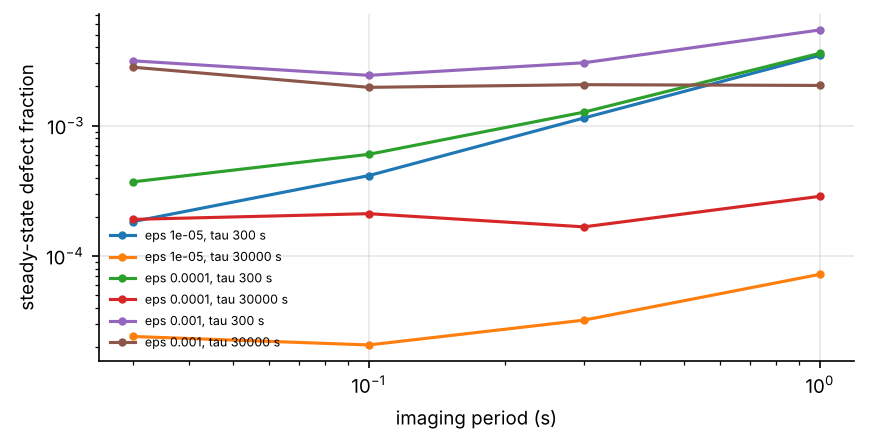
\includegraphics[width=0.8\linewidth]{m25_imaging.png}
\caption{Steady-state defect fraction sampled just after each image versus imaging period, at $10^5$ sites (4~$\times$~4~\textmu m, 85\% loading, 32~$\times$~4 block, intermediate steps, $t_\mathrm{img}=10$~ms, loss $10^{-4}$ per move), for $\epsilon_\mathrm{img}=10^{-5}$, $10^{-4}$, $10^{-3}$ and $\tau=300$ and 30000~s. Each point is one seed, averaged over the second half of a run of $\max(8~\mathrm{s},8T_\mathrm{img})$. The full scan (with $\tau=3000$~s) fits $\rho_\mathrm{image}=2.24\epsilon_\mathrm{img}+0.98(T_\mathrm{img}+t_\mathrm{img})/\tau$; time averages are in Table~\ref{tab:mega-imaging}.}
\label{fig:mega-imaging}
\end{figure}

The time average follows a hole-lifetime model. Let $T=T_\mathrm{img}+t_\mathrm{img}$. An imaging loss is unseen for one period $T$ and is then repaired after a mean delay $d$; a vacuum loss waits $T/2$ on average for the next image, and then $d$. Hence
\begin{equation}
\rho_\mathrm{mean}=\epsilon_\mathrm{img}\,\frac{T+d}{T}+\frac{T/2+d}{\tau}.
\end{equation}
One delay, $d=22$~ms, fits all 40 points at $10^5$ sites with a median error of 9\% ($d=0$ underestimates by a median 16\%). The worst point (41\%) is $\epsilon_\mathrm{img}=10^{-3}$ at $T_\mathrm{img}=30$~ms, where the repair saturates. Minimising $\rho_\mathrm{mean}$ over $T$ gives the optimum imaging period
\begin{equation}
T^*=\sqrt{2\,\epsilon_\mathrm{img}\,d\,\tau}\qquad(d\ll T).
\end{equation}
For $d=22$~ms and $\tau=3000$~s this is 36~ms, 0.11~s and 0.36~s for $\epsilon_\mathrm{img}=10^{-5}$, $10^{-4}$ and $10^{-3}$, in agreement with the minima of the scan (0.03~s, 0.1~s, and a flat minimum between 0.3 and 1~s). At the optimum, $\rho_\mathrm{mean}\approx\epsilon_\mathrm{img}+\sqrt{2\epsilon_\mathrm{img}d/\tau}+d/\tau$; for $\epsilon_\mathrm{img}=10^{-4}$ and $\tau=3000$~s that is $1.5\times10^{-4}$ (simulated $1.4\times10^{-4}$ at $T_\mathrm{img}=0.1$~s). Hence the loss per image dominates the floor once $\tau$ exceeds a few thousand seconds, and lowering $\epsilon_\mathrm{img}$, not imaging more often, is the lever. The imaging time matters only through the dead time at short periods: at $T_\mathrm{img}=30$~ms, $t_\mathrm{img}=3$, 10 and 20~ms give $1.28$, $1.48$ and $1.66\times10^{-4}$.

At $10^6$ sites the delay is not a constant, because the block must sweep its positions to reach a hole (252 for a 32~$\times$~4 block on 4~$\times$~4~\textmu m; a one-pass visit takes 0.9 to 1.0~ms with fast steps and 1.35 to 1.5~ms with intermediate steps). Table~\ref{tab:mega-imaging6} gives the time averages for $\epsilon_\mathrm{img}=10^{-4}$ and $\tau=3000$~s. At $T_\mathrm{img}=30$~ms both timings saturate. The loss rate, $\epsilon_\mathrm{img}/T+1/\tau=2.8\times10^{-3}$ per site per second, needs 2,800 fills per second. At $\rho=2\times10^{-4}$ a block position holds about 0.8 holes, so a sweep of 252 visits (0.25 to 0.4~s) refills only about 200 atoms, while the imaging dead time takes 25\% of the time; the holes pile up until each visit has enough work. By Little's law the mean hole lifetime is $\rho_\mathrm{mean}/(\epsilon_\mathrm{img}/T+1/\tau)$: 0.15~s for fast steps at $T_\mathrm{img}=0.1$~s, and 0.33~s for intermediate steps at both 0.1 and 0.3~s. Intermediate steps at $T_\mathrm{img}=0.3$~s thus reach $2.2\times10^{-4}$, within 15\% of fast steps at 0.1~s, with the 128-engine block and one fifth of the heating per refilled atom (2 against 10~\textmu K). At $10^6$ sites a slower imaging cadence is therefore an alternative to a larger block: the imaging period should match the sweep time of the block rather than be as short as possible.

\begin{table}[htbp]\centering\small
\caption{Time-averaged defect fraction at $10^6$ sites with the 32~$\times$~4 block, $\epsilon_\mathrm{img}=10^{-4}$, $\tau=3000$~s (simulated, \texttt{results/\allowbreak m25\_imaging.json}).}
\label{tab:mega-imaging6}
\begin{tabular}{lccc}
\toprule
timing & $T_\mathrm{img}=0.03$~s & 0.1~s & 0.3~s \\
\midrule
fast (10~\textmu K per move) & $8.7\times10^{-4}$ & $1.9\times10^{-4}$ & $2.0\times10^{-4}$ \\
intermediate (2~\textmu K per move) & $1.5\times10^{-3}$ & $4.1\times10^{-4}$ & $2.2\times10^{-4}$ \\
\bottomrule
\end{tabular}
\end{table}

\subsection{Limits}\label{sec:megascale-limits}

The steady-state model assumes perfect detection apart from the imaging loss, an external reservoir supply, a single objective whose field reaches every site, and one move per refill. It does not schedule the reservoir refresh physically (conveyor timing) and does not include photon scattering. The heating per move is taken from the 1D quantum and 3D classical transport results (Sec.~\ref{sec:transport}), not computed within the steady-state model. The remedy and imaging scans use one seed per case. The tiling result is 1D, with ideal thin lenslets and no surface scatter, and the 24~mm chip edge for a 32~$\times$~8 block is not designed. The static-potential comparison is a first-order budget with an assumed delivery efficiency and cavity buildup. Recommendations follow directly. For $10^4$ sites, one large-field objective or two zones and one 16-chip stack suffice. For $10^5$ sites, a 32~$\times$~4 block, a field of $\pm0.9$~mm or about 13 zones, and about 85\% loading, which cuts the reservoir from two thirds of the sites to a quarter and the static power by 40\%. For $10^6$ sites the transport side is feasible with a block of 128 to 256 engines, but the static potential needs a different source (a cavity lattice or much lower depths), the field needs a lithography-class objective, and the loss rates must improve to reach $10^{-4}$ defects.
